\begin{solution}{normal}\textbf{(a)} In analogy to electrical circuits, the resistance of a single wire is given by:
$$R = \frac{L}{\kappa S}$$
Since we have four wires in parallel, the effective resistance is:
$$R = \frac{L}{4\kappa S}$$
\vspace{3mm}

\noindent \textbf{(b)} For a small period of time $\text{d}t$, the temperature is changed by $\Delta T$ degrees. This means that 
\[P \equiv \frac{\text{d}Q}{\text{d}t} = C\Delta\dot{T}.\]
Let us look at the electrical analogy between heat conduction and electric circuits. In this case, $\dot{Q}$ acts as the current while the temperature difference $\Delta T \equiv T - T_0$ acts as the voltage difference. From this perspective, we can also define 
\[\dot{Q} = \frac{\Delta T}{R}.\]
This means that from adding these two individual expressions (as there is an extra $\dot{Q}$ due to our "voltage difference") we have that 
\[P\cos \omega t = C\Delta\dot{T} + \frac{\Delta T}{R}.\]
As power varies with time, we attempt to seek the solution in the form of 
\[T = T_0 + \Delta T \sin (\omega t + \phi).\]
Taking the derivative of our sought solution and substituting into our differential equation gives us 
\[P\cos\omega t = C\Delta T\omega \cos (\omega t + \phi) + \frac{\Delta T}{R}\cos \left(\omega t + \phi - \frac{\pi}{2}\right)\]
which can be seen as the sum of multiple rotating vectors or:
\[\vec{P} = \vec{P}_C + \vec{P}_R.\]
Each of these vectors have an individual magnitude of 
\[P_C = C\Delta T \omega, \quad P_R = \frac{\Delta T}{R}\]
\begin{center}
    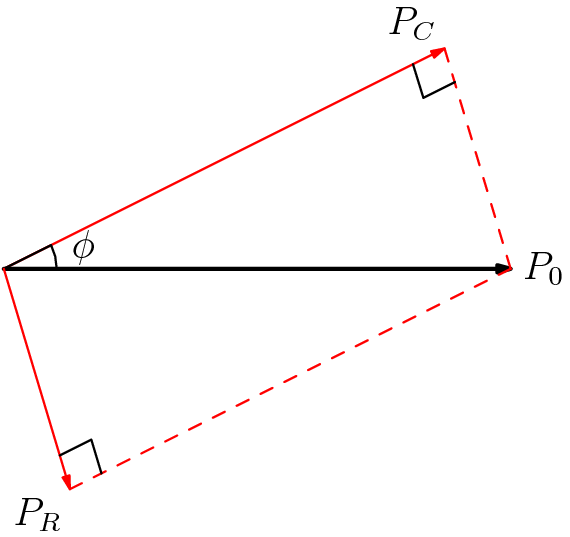
\includegraphics[width=6cm]{phasor.png}
\end{center}
Therefore, from pythagorean theorem, the amplitude of oscillations is 
\[P_0^2 = (C\omega\Delta T)^2 + \left(\frac{\Delta T}{R}\right)^2\implies \Delta T = \frac{P_0}{\sqrt{C^2\omega^2 + R^{-2}}}.\]
Our solution is in the form of 
\[T = T_0 + \Delta T \sin (\omega t + \phi) = T_0 +  \frac{P_0\cos (\omega t + \phi)}{\sqrt{C^2\omega^2 + R^{-2}}}.\]
Let us estimate the phase difference. We can go back to our phase diagram and see that 
\[\phi = \arcsin\left(\frac{P_C}{P_0}\right) = \arcsin\left(\frac{C\omega}{\sqrt{C^2 \omega^2 + R^{-2}}}\right).\]
This means that our final solution is 
\[T = T_0 +  \frac{P_0\cos \left(\omega t + \arcsin\left(C\omega/\sqrt{C^2 \omega^2 + R^{-2}}\right)\right)}{\sqrt{C^2\omega^2 + R^{-2}}} .\]
\vspace{3mm}

\noindent \textbf{(c)} Remember from part b that our amplitude of oscillations of $\Delta T$ is given by $\Delta T = \frac{P_0}{\sqrt{C^2\omega^2 + R^{-2}}}$. We want there to be as large a change as possible with a small change in $C$. This is equivalent to maximizing the derivative ie setting the double derivative to $0$. Upon taking two derivatives, we get the function
\[\frac{3P_0 C^2 \omega^4}{(C^2 \omega^2 + R^{-2})^{5/2}} - \frac{P_0 \omega^2}{(C^2 \omega^2 + R^{-2})^{3/2}} = 0.\]
Seperating and solving for $\omega$ yields $\omega = 1/\sqrt{2}CR$.
\vspace{3mm}

\noindent \textbf{(d)} As the questions asks to estimate, we ignore all numerical prefactors. From part c), we know that $C \approx 1/\omega R$. This should be of the same order as the heat capacity of the bridges. Therefore, we have 
\[\frac{1}{l/\kappa S\cdot \omega} = \rho lSc\implies \omega_c \approx \frac{\kappa}{c\rho L^2}.\]
\end{solution}